\documentclass[8pt,aspectratio=169]{beamer}
\usetheme{Madrid}
\usepackage{graphicx}
\usepackage{booktabs}
\usepackage{adjustbox}
\usepackage{multicol}
\usepackage{amsmath}
\usepackage{amssymb}
\usepackage{tikz}
\usepackage{hyperref}
\usepackage{algorithm}
\usepackage{algorithmic}
\usepackage{colortbl}
\usepackage{pgfplots}
\pgfplotsset{compat=1.18}

% TikZ libraries for comics, diagrams, stakeholder maps
\usetikzlibrary{arrows.meta,positioning,shapes.callouts,shapes.geometric,decorations.pathreplacing}

% Color definitions
\definecolor{mlblue}{RGB}{0,102,204}
\definecolor{mlpurple}{RGB}{51,51,178}
\definecolor{mllavender}{RGB}{173,173,224}
\definecolor{mllavender2}{RGB}{193,193,232}
\definecolor{mllavender3}{RGB}{204,204,235}
\definecolor{mllavender4}{RGB}{214,214,239}
\definecolor{mlorange}{RGB}{255, 127, 14}
\definecolor{mlgreen}{RGB}{44, 160, 44}
\definecolor{mlred}{RGB}{214, 39, 40}
\definecolor{mlgray}{RGB}{127, 127, 127}
\definecolor{lightgray}{RGB}{240, 240, 240}
\definecolor{midgray}{RGB}{180, 180, 180}

% NEW COLORS for mini-lecture
\definecolor{dfteal}{RGB}{0,128,128}
\definecolor{dfred}{RGB}{180,30,30}

% Backward compatibility
\colorlet{MLPurple}{mlpurple}
\colorlet{MLBlue}{mlblue}
\colorlet{MLOrange}{mlorange}
\colorlet{MLGreen}{mlgreen}
\colorlet{MLRed}{mlred}
\colorlet{MLLavender}{mllavender}
\colorlet{MLGray}{mlgray}

% Theme colors (exact Madrid settings)
\setbeamercolor{palette primary}{bg=mllavender3,fg=mlpurple}
\setbeamercolor{palette secondary}{bg=mllavender2,fg=mlpurple}
\setbeamercolor{palette tertiary}{bg=mllavender,fg=white}
\setbeamercolor{palette quaternary}{bg=mlpurple,fg=white}
\setbeamercolor{structure}{fg=mlpurple}
\setbeamercolor{section in toc}{fg=mlpurple}
\setbeamercolor{subsection in toc}{fg=mlblue}
\setbeamercolor{title}{fg=mlpurple}
\setbeamercolor{frametitle}{fg=mlpurple,bg=mllavender3}
\setbeamercolor{block title}{bg=mllavender2,fg=mlpurple}
\setbeamercolor{block body}{bg=mllavender4,fg=black}
\setbeamertemplate{navigation symbols}{}
\setbeamertemplate{itemize items}[circle]
\setbeamertemplate{enumerate items}[default]
\setbeamersize{text margin left=5mm,text margin right=5mm}

% Footer
\setbeamertemplate{footline}{
  \leavevmode%
  \hbox{%
    \begin{beamercolorbox}[wd=.333333\paperwidth,ht=2.25ex,dp=1ex,center]{author in head/foot}%
      \usebeamerfont{author in head/foot}Methods and Algorithms
    \end{beamercolorbox}%
    \begin{beamercolorbox}[wd=.333333\paperwidth,ht=2.25ex,dp=1ex,center]{title in head/foot}%
      \usebeamerfont{title in head/foot}MSc Data Science
    \end{beamercolorbox}%
    \begin{beamercolorbox}[wd=.333333\paperwidth,ht=2.25ex,dp=1ex,right]{date in head/foot}%
      \usebeamerfont{date in head/foot}\insertframenumber{} / \inserttotalframenumber\hspace*{2ex}
    \end{beamercolorbox}}%
  \vskip0pt%
}

\newcommand{\bottomnote}[1]{%
\vfill
\vspace{-2mm}
\textcolor{mllavender2}{\rule{\textwidth}{0.4pt}}
\vspace{1mm}
\footnotesize
\textbf{#1}
}

\newenvironment{compactlist}{%
  \begin{itemize}%
    \setlength{\itemsep}{2pt}%
    \setlength{\parskip}{0pt}%
    \setlength{\parsep}{0pt}%
}{%
  \end{itemize}%
}

\newcommand{\highlight}[1]{\textcolor{mlorange}{\textbf{#1}}}
\newcommand{\mathbold}[1]{\boldsymbol{#1}}

% =====================================================
\title[Embeddings Full Lecture]{Word Embeddings}
\subtitle{Teaching Machines to Understand Language}
\author{Methods \& Algorithms}
\date{MSc Data Science -- Spring 2026}

\begin{document}

% =====================================================
% INTRO ZONE (slides 1-5, NO formulas)
% =====================================================

% --- Slide 1: Title ---
\begin{frame}
\titlepage
\end{frame}

% --- Slide 2: Opening Comic ---
\begin{frame}{How Would You Teach a Computer What ``Bullish'' Means?}
\centering
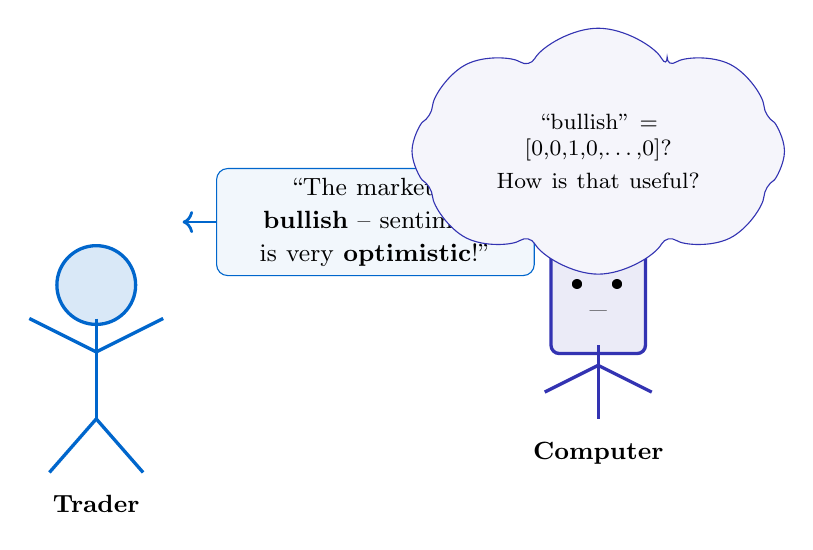
\begin{tikzpicture}[scale=0.85]
  % Trader
  \node[circle, draw=mlblue, fill=mlblue!15, minimum size=1cm, line width=1.2pt] (trader) at (-2.5,2) {};
  \draw[mlblue, line width=1.2pt] (-2.5,1.5) -- (-2.5,0);
  \draw[mlblue, line width=1.2pt] (-2.5,1) -- (-3.5,1.5);
  \draw[mlblue, line width=1.2pt] (-2.5,1) -- (-1.5,1.5);
  \draw[mlblue, line width=1.2pt] (-2.5,0) -- (-3.2,-0.8);
  \draw[mlblue, line width=1.2pt] (-2.5,0) -- (-1.8,-0.8);
  \node[below] at (-2.5,-1) {\small\textbf{Trader}};
  % Speech bubble
  \node[draw=mlblue, fill=mlblue!5, rounded corners=4pt, text width=3.8cm,
        align=center, right=1cm of trader, yshift=0.8cm] (speech)
        {\small ``The market is \textbf{bullish} -- sentiment is very \textbf{optimistic}!''};
  \draw[->,mlblue,line width=1pt] (speech.west) -- +(-0.5,0);
  % Robot
  \node[draw=mlpurple, fill=mlpurple!10, rounded corners=3pt,
        minimum width=1.2cm, minimum height=1.4cm, line width=1.2pt] (robot) at (5,1.8) {};
  \node at (4.7,2) {\small\textbullet};
  \node at (5.3,2) {\small\textbullet};
  \node at (5,1.6) {\tiny ---};
  \draw[mlpurple, line width=1.2pt] (5,1.1) -- (5,0);
  \draw[mlpurple, line width=1.2pt] (5,0.8) -- (4.2,0.4);
  \draw[mlpurple, line width=1.2pt] (5,0.8) -- (5.8,0.4);
  \node[below] at (5,-0.2) {\small\textbf{Computer}};
  % Thought bubble
  \node[draw=mlpurple, fill=mlpurple!5, rounded corners=4pt, cloud, cloud puffs=8,
        cloud puff arc=120, aspect=2, text width=3cm, align=center]
        at (5,4) {\footnotesize ``bullish'' = [0,0,1,0,\ldots,0]?\\ How is that useful?};
\end{tikzpicture}

\bottomnote{Words are just strings -- how do we make them mathematical?}
\end{frame}

% --- Slide 3: Learning Objectives ---
\begin{frame}{Learning Objectives}
After this lecture, you will be able to:
\begin{enumerate}
  \item \textbf{Derive} the Skip-gram objective and explain negative sampling
  \item \textbf{Analyze} embedding spaces using cosine similarity and analogy tasks
  \item \textbf{Evaluate} Word2Vec vs GloVe vs contextual embeddings
  \item \textbf{Apply} embeddings to financial sentiment analysis
\end{enumerate}

\bottomnote{LOs at Bloom's levels 4--5: analyze, evaluate, apply, derive.}
\end{frame}

% --- Slide 4: What Is a Word Embedding? ---
\begin{frame}{What Is a Word Embedding?}
\begin{columns}[T]
\begin{column}{0.52\textwidth}
A \highlight{word embedding} maps words to dense vectors where
\textbf{similar words have similar vectors}.

\vspace{4pt}
\begin{compactlist}
  \item Each word $\rightarrow$ real-valued vector in $\mathbb{R}^d$
  \item Typical $d$: 50--300 dimensions
  \item Famous analogy: \texttt{king} $-$ \texttt{man} $+$ \texttt{woman} $\approx$ \texttt{queen}
\end{compactlist}
\end{column}
\begin{column}{0.45\textwidth}
\begin{block}{Key Terms}
\begin{compactlist}
  \item \textbf{Embedding}: learned vector representation
  \item \textbf{Dense vector}: most entries non-zero
  \item \textbf{Cosine similarity}: measures vector closeness
\end{compactlist}
\end{block}
\end{column}
\end{columns}

\bottomnote{Embeddings turn words into numbers that capture meaning.}
\end{frame}

% --- Slide 5: Why Not One-Hot? ---
\begin{frame}{Why Not Just Use One-Hot Encoding?}
\begin{columns}[T]
\begin{column}{0.48\textwidth}
\textbf{One-Hot Encoding}
\begin{compactlist}
  \item Dimension = vocabulary size ($V \sim 100$K)
  \item Every word equally distant from every other
  \item ``bullish'' and ``optimistic'' are orthogonal
\end{compactlist}
\end{column}
\begin{column}{0.48\textwidth}
\textbf{Dense Embeddings}
\begin{compactlist}
  \item Dimension = 50--300 (compact)
  \item Similar words are nearby in vector space
  \item ``bullish'' $\approx$ ``optimistic'' by cosine similarity
\end{compactlist}
\end{column}
\end{columns}

\bottomnote{One-hot: sparse and meaningless distances. Embeddings: dense and semantic.}
\end{frame}

% =====================================================
% CORE -- METHOD (slides 6-14)
% =====================================================

% --- Slide 6: Embedding Space (chart) ---
\begin{frame}{What Does the Embedding Space Look Like?}
\centering

\includegraphics[width=0.65\textwidth]{01_word_embedding_space/chart.pdf}

\bottomnote{Words with related meanings cluster together in embedding space.}
\end{frame}

% --- Slide 7: Distributional Hypothesis ---
\begin{frame}{The Distributional Hypothesis}
\begin{block}{Core Idea (Firth, 1957)}
``You shall know a word by the company it keeps.''
\end{block}

\vspace{6pt}
\begin{compactlist}
  \item Words appearing in \textbf{similar contexts} have \textbf{similar meanings}
  \item ``The stock \underline{\hspace{1cm}} sharply today'' $\rightarrow$ rose, fell, rallied, plunged
  \item Context windows capture co-occurrence patterns
\end{compactlist}

\bottomnote{The distributional hypothesis is the foundation of all embedding methods.}
\end{frame}

% --- Slide 8: Skip-gram Architecture (chart) ---
\begin{frame}{Skip-gram: Predicting Context from a Word}
\begin{columns}[T]
\begin{column}{0.48\textwidth}
\begin{compactlist}
  \item Given a \highlight{center word}, predict surrounding context words
  \item Window size $c$ controls how far to look
  \item The hidden layer weights \textbf{become} the embeddings
\end{compactlist}
\end{column}
\begin{column}{0.48\textwidth}

\includegraphics[width=\textwidth]{08_skipgram_architecture/chart.pdf}
\end{column}
\end{columns}

\bottomnote{Skip-gram learns embeddings by predicting which words appear nearby.}
\end{frame}

% --- Slide 9: Skip-gram Objective ---
\begin{frame}{The Skip-gram Objective}
Maximize the average log-probability of context words:
\[
  \max_{\theta}\; \frac{1}{T}\sum_{t=1}^{T}\sum_{\substack{-c \le j \le c \\ j\neq 0}} \log p(w_{t+j} \mid w_t)
\]

where the softmax over the full vocabulary defines:
\[
  p(w_O \mid w_I) = \frac{\exp\!\bigl(\mathbf{v}'_{w_O} \!\cdot\! \mathbf{v}_{w_I}\bigr)}{\sum_{w=1}^{V}\exp\!\bigl(\mathbf{v}'_w \!\cdot\! \mathbf{v}_{w_I}\bigr)}
\]

\begin{compactlist}
  \item $T$ = number of words in the corpus, $c$ = context window
  \item Denominator sums over \textbf{entire vocabulary} -- prohibitively expensive!
\end{compactlist}

\bottomnote{The softmax normalization costs $O(V)$ per update -- we need a shortcut.}
\end{frame}

% --- Slide 10: Negative Sampling (chart) ---
\begin{frame}{Negative Sampling: Making Training Feasible}
\begin{columns}[T]
\begin{column}{0.48\textwidth}
Instead of softmax over $V$ words, sample $k$ \highlight{negative} examples:
\[
  \log \sigma(\mathbf{v}'_{w_O}\!\cdot\!\mathbf{v}_{w_I}) + \sum_{i=1}^{k}\mathbb{E}\bigl[\log \sigma(-\mathbf{v}'_{w_i}\!\cdot\!\mathbf{v}_{w_I})\bigr]
\]
\begin{compactlist}
  \item Positive pair: real context word
  \item Negative pairs: $k$ random words
  \item Typical $k$: 5--20
\end{compactlist}
\end{column}
\begin{column}{0.48\textwidth}

\includegraphics[width=\textwidth]{10_negative_sampling/chart.pdf}
\end{column}
\end{columns}

\bottomnote{Negative sampling reduces cost from $O(V)$ to $O(k)$ per update.}
\end{frame}

% --- Slide 11: Cosine Similarity (chart) ---
\begin{frame}{Measuring Similarity: Cosine Distance}
\begin{columns}[T]
\begin{column}{0.48\textwidth}
\[
  \cos(\mathbf{a}, \mathbf{b}) = \frac{\mathbf{a} \cdot \mathbf{b}}{\|\mathbf{a}\|\;\|\mathbf{b}\|}
\]
\begin{compactlist}
  \item $+1$: identical direction (synonyms)
  \item $0$: orthogonal (unrelated)
  \item $-1$: opposite (antonyms, sometimes)
\end{compactlist}
\end{column}
\begin{column}{0.48\textwidth}

\includegraphics[width=\textwidth]{02_similarity_heatmap/chart.pdf}
\end{column}
\end{columns}

\bottomnote{Cosine similarity is the standard metric for comparing word embeddings.}
\end{frame}

% --- Slide 12: Word Analogies ---
\begin{frame}{Word Analogies: The Magic of Vector Arithmetic}
\begin{block}{Worked Example}
$\texttt{king} - \texttt{man} + \texttt{woman} \approx \texttt{queen}$
\end{block}

\vspace{4pt}
\textbf{Step-by-step} (simplified 3D vectors):

\begin{compactlist}
  \item $\mathbf{v}_{\text{king}} = [0.9, 0.7, 0.1]$, \;
        $\mathbf{v}_{\text{man}} = [0.8, 0.1, 0.1]$, \;
        $\mathbf{v}_{\text{woman}} = [0.8, 0.1, 0.9]$
  \item $\mathbf{v}_{\text{king}} - \mathbf{v}_{\text{man}} + \mathbf{v}_{\text{woman}} = [0.9, 0.7, 0.9]$
  \item Nearest neighbor: $\texttt{queen} = [0.9, 0.7, 0.85]$ \checkmark
\end{compactlist}

\vspace{4pt}
\textbf{Finance analogy:} $\texttt{stock} - \texttt{equity} + \texttt{debt} \approx \texttt{bond}$

\bottomnote{Vector arithmetic captures relational structure: gender, asset class, and more.}
\end{frame}

% --- Slide 13: GloVe ---
\begin{frame}{GloVe: Global Vectors from Co-occurrence}
\begin{columns}[T]
\begin{column}{0.48\textwidth}
GloVe minimizes a weighted least-squares objective on the
\textbf{log co-occurrence matrix}:
\[
  \sum_{i,j} f(X_{ij})\bigl(\mathbf{w}_i \!\cdot\! \tilde{\mathbf{w}}_j + b_i + \tilde{b}_j - \log X_{ij}\bigr)^2
\]
\begin{compactlist}
  \item $X_{ij}$: how often word $i$ appears near word $j$
  \item $f$: weighting function (caps frequent pairs)
\end{compactlist}
\end{column}
\begin{column}{0.48\textwidth}
\begin{block}{Skip-gram vs GloVe}
\small
\begin{tabular}{lll}
\toprule
& \textbf{Skip-gram} & \textbf{GloVe} \\
\midrule
Type & Predictive & Count-based \\
Input & Local windows & Global matrix \\
Speed & Online & Batch \\
\bottomrule
\end{tabular}
\end{block}
\end{column}
\end{columns}

\bottomnote{GloVe combines the efficiency of matrix factorization with the quality of prediction-based methods.}
\end{frame}

% --- Slide 14: Decision Flowchart (chart) ---
\begin{frame}{When to Use Which Approach?}
\begin{columns}[T]
\begin{column}{0.42\textwidth}
\begin{compactlist}
  \item \textbf{Small corpus}: use pre-trained GloVe or Word2Vec
  \item \textbf{Domain-specific}: fine-tune on your data
  \item \textbf{Context matters}: use BERT / contextual models
\end{compactlist}
\end{column}
\begin{column}{0.55\textwidth}

\includegraphics[width=\textwidth]{07_decision_flowchart/chart.pdf}
\end{column}
\end{columns}

\bottomnote{The right embedding method depends on corpus size, domain, and task requirements.}
\end{frame}

% =====================================================
% CORE -- SOLUTION (slides 15-19)
% =====================================================

% --- Slide 15: Financial Sentiment ---
\begin{frame}{Financial Sentiment Analysis with Embeddings}
\begin{columns}[T]
\begin{column}{0.48\textwidth}
\textbf{Approach}
\begin{compactlist}
  \item Train Word2Vec on financial news corpus
  \item Embedding space reveals sentiment clusters
  \item Use clusters as features for a classifier
\end{compactlist}
\end{column}
\begin{column}{0.48\textwidth}
\textbf{Observed Clusters}
\begin{compactlist}
  \item \textcolor{mlgreen}{Bullish}: rally, surge, upgrade, outperform
  \item \textcolor{mlred}{Bearish}: crash, plunge, downgrade, miss
  \item \textcolor{mlblue}{Neutral}: report, announce, file, disclose
\end{compactlist}
\end{column}
\end{columns}

\bottomnote{Word2Vec on domain text captures financial sentiment without manual labeling.}
\end{frame}

% --- Slide 16: Document Vectors ---
\begin{frame}{From Words to Documents: Averaging Embeddings}
\textbf{Step-by-step:}
\begin{enumerate}
  \item Look up each word's embedding: $\mathbf{v}_{w_1}, \mathbf{v}_{w_2}, \ldots, \mathbf{v}_{w_n}$
  \item Compute the document vector: $\mathbf{d} = \frac{1}{n}\sum_{i=1}^{n} \mathbf{v}_{w_i}$
  \item \textit{Optional}: weight by TF-IDF to emphasize important terms
\end{enumerate}

\vspace{4pt}
\textbf{Example}: Average embedding of an earnings call transcript
$\rightarrow$ single vector $\rightarrow$ sentiment score via logistic regression.

\bottomnote{Simple averaging is a strong baseline -- often competitive with more complex methods.}
\end{frame}

% --- Slide 17: Contextual Embeddings ---
\begin{frame}{Contextual Embeddings: BERT and Beyond}
\small
\begin{tabular}{p{2.5cm}p{4.5cm}p{4.5cm}}
\toprule
& \textbf{Static (Word2Vec, GloVe)} & \textbf{Contextual (BERT, GPT)} \\
\midrule
Same word & Same vector always & Different vector per context \\
``bank'' & One vector for all uses & ``river bank'' $\neq$ ``investment bank'' \\
Training & Unsupervised, fast & Pre-trained, fine-tuned \\
Size & 50--300 dims & 768--1024 dims \\
Best for & Simple tasks, speed & Disambiguation, QA, NER \\
\bottomrule
\end{tabular}

\bottomnote{Contextual embeddings solve polysemy but require more compute.}
\end{frame}

% --- Slide 18: Embeddings as Preprocessing ---
\begin{frame}[fragile]{Embeddings as Preprocessing for ML}
\small
\begin{verbatim}
from sklearn.pipeline import Pipeline
from sklearn.feature_extraction.text import TfidfVectorizer
from sklearn.decomposition import TruncatedSVD
from sklearn.linear_model import LogisticRegression

pipe = Pipeline([
    ('tfidf', TfidfVectorizer(max_features=5000)),
    ('svd',   TruncatedSVD(n_components=50)),
    ('clf',   LogisticRegression())
])
pipe.fit(X_train, y_train)
print(f"Accuracy: {pipe.score(X_test, y_test):.3f}")
\end{verbatim}

\bottomnote{TF-IDF + SVD is a simple, effective embedding pipeline for text classification.}
\end{frame}

% --- Slide 19: NER in Finance ---
\begin{frame}{Named Entity Recognition in Finance}
\begin{columns}[T]
\begin{column}{0.48\textwidth}
\textbf{Embedding-Based NER}
\begin{compactlist}
  \item Identify company names, tickers, monetary amounts
  \item Embeddings learn that ``AAPL'' and ``Apple'' are related
  \item Context resolves ``Apple'' (company vs fruit)
\end{compactlist}
\end{column}
\begin{column}{0.48\textwidth}
\textbf{Example Entities}
\begin{compactlist}
  \item \textcolor{mlblue}{ORG}: Goldman Sachs, JPMorgan
  \item \textcolor{mlgreen}{TICKER}: AAPL, TSLA, MSFT
  \item \textcolor{mlorange}{MONEY}: \$2.5B, EUR 140M
\end{compactlist}
\end{column}
\end{columns}

\bottomnote{Pre-trained embeddings + fine-tuning deliver strong NER on financial text.}
\end{frame}

% =====================================================
% CLOSING (slides 20-25)
% =====================================================

% --- Slide 20: When to Use ---
\begin{frame}{When to Use Embeddings -- and When Not To}
\begin{columns}[T]
\begin{column}{0.48\textwidth}
\textbf{\textcolor{mlgreen}{Pros}}
\begin{compactlist}
  \item Capture semantic similarity
  \item Transfer learning from large corpora
  \item Compact representation (50--300 dims)
\end{compactlist}
\end{column}
\begin{column}{0.48\textwidth}
\textbf{\textcolor{mlred}{Cons}}
\begin{compactlist}
  \item Need large corpus to train well
  \item Not interpretable (black-box vectors)
  \item Static models ignore context
\end{compactlist}
\end{column}
\end{columns}

\bottomnote{Use pre-trained embeddings when your corpus is small; fine-tune when domain matters.}
\end{frame}

% --- Slide 21: Comparison Table ---
\begin{frame}{Embeddings vs Bag-of-Words vs TF-IDF}
\small
\begin{tabular}{p{2.5cm}p{3cm}p{3cm}p{3cm}}
\toprule
& \textbf{Bag-of-Words} & \textbf{TF-IDF} & \textbf{Embeddings} \\
\midrule
Sparsity & Very sparse & Sparse & Dense \\
Semantics & None & Term importance & Full similarity \\
Dimensions & $V$ (large) & $V$ (large) & 50--300 \\
Training data & None needed & None needed & Large corpus \\
Interpretable & Yes & Yes & No \\
\bottomrule
\end{tabular}

\bottomnote{Each representation makes a different trade-off between simplicity and expressiveness.}
\end{frame}

% --- Slide 22: Hands-on ---
\begin{frame}[fragile]{Hands-on: Explore Financial Word Vectors}
\small
\begin{verbatim}
import numpy as np
from sklearn.metrics.pairwise import cosine_similarity

# Hand-crafted finance embeddings (3D for illustration)
words = ['stock','bond','equity','debt','rally','crash']
vecs = np.array([[0.9,0.2,0.1],[0.1,0.9,0.2],
                 [0.85,0.15,0.1],[0.15,0.85,0.25],
                 [0.7,0.1,0.8],[0.7,0.1,-0.8]])

sim = cosine_similarity(vecs)
print("Similarity: stock-equity =", f"{sim[0,2]:.3f}")
print("Similarity: stock-crash  =", f"{sim[0,5]:.3f}")
\end{verbatim}
\vspace{2pt}
\small Full notebook: \texttt{L06\_embeddings.ipynb}

\bottomnote{Try the notebook to explore embedding spaces interactively.}
\end{frame}

% --- Slide 23: Key Takeaways ---
\begin{frame}{Key Takeaways}
\begin{columns}[T]
\begin{column}{0.48\textwidth}
\textbf{Concepts}
\begin{compactlist}
  \item Distributional hypothesis drives all embeddings
  \item Skip-gram + negative sampling = efficient training
  \item Cosine similarity measures semantic closeness
  \item GloVe combines local and global statistics
\end{compactlist}
\end{column}
\begin{column}{0.48\textwidth}
\textbf{Practice}
\begin{compactlist}
  \item Pre-trained $>$ train-your-own (usually)
  \item Check analogies to validate quality
  \item Use BERT when context matters
  \item TF-IDF + SVD is a strong baseline
\end{compactlist}
\end{column}
\end{columns}

\bottomnote{Embeddings are the bridge between raw text and machine learning.}
\end{frame}

% --- Slide 24: Bridge ---
\begin{frame}{What's Next: Reinforcement Learning}
\begin{compactlist}
  \item Embeddings teach machines to \textbf{represent} language
  \item Reinforcement learning teaches machines to \textbf{act}
  \item Next: how agents learn optimal strategies from rewards
\end{compactlist}

\vspace{8pt}
\centering
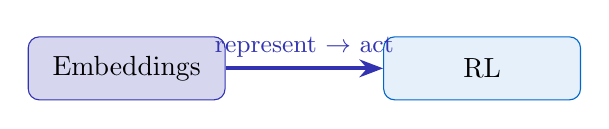
\begin{tikzpicture}
  \node[draw=mlpurple, fill=mllavender4, rounded corners, minimum width=2.5cm, minimum height=0.8cm] (emb) {Embeddings};
  \node[draw=mlblue, fill=mlblue!10, rounded corners, minimum width=2.5cm, minimum height=0.8cm, right=2cm of emb] (rl) {RL};
  \draw[-{Stealth[length=3mm]}, line width=1.5pt, mlpurple] (emb) -- node[above]{\small represent $\rightarrow$ act} (rl);
\end{tikzpicture}

\bottomnote{From understanding language to making decisions under uncertainty.}
\end{frame}

% --- Slide 25: Closing ---
\begin{frame}{Closing Thought}
\centering
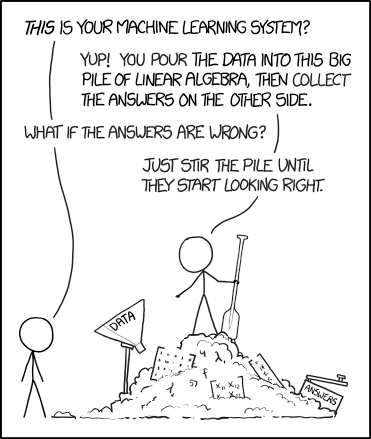
\includegraphics[width=0.6\textwidth,height=0.7\textheight,keepaspectratio]{images/1838_machine_learning.png}

\bottomnote{XKCD \#1838 by Randall Munroe (CC BY-NC 2.5)}
\end{frame}

\end{document}
